\chapter{Agent Implementation Instructions}\label{ch:agent-impl}

\section{Purpose and audience}
This chapter is the self-contained, intent-based instruction set for
implementing the \emph{Regulations} domain inside the unified SAP
OSS platform. Regulations plays two roles at once: it is a persona
surface (Compliance Officer) in its own right, \emph{and} it is the
horizontal runtime wrapper that governs the three other domains
(Arabic AP, TB, Simula) at every MCP call. This chapter is written
for LLM-driven and human implementation agents who will extend
existing services to realise both roles. It assumes only this PDF;
every platform decision, integration contract, and governance
obligation is restated here so that no companion document is
required. Existing chapters~\ref{ch:overview}--\ref{ch:reg-roadmap}
remain the normative source for the regulations domain itself; this
chapter tells future agents \emph{how} to build what those chapters
describe, \emph{where} to put it in the codebase, and \emph{how} it
plugs into the wider platform.

% !TEX root = ../master.tex
% =============================================================================
% MASTER PLATFORM CORE: Shared Intent-Based Instructions (Union)
% World-Class Version: HITL Gates, Process Integrity, and .clinerules Wiring
% =============================================================================

\section{Rules of Engagement for AI Agents}
\label{sec:agent-rules}

To ensure safety and architectural integrity, all implementation agents must adhere to the following Prime Directives:

\begin{enumerate}[label=\textsc{rule}-\arabic*:, leftmargin=2cm]
    \item \textbf{Credential Protection.} Never log, print, or commit secrets. Use the \texttt{.secrets.example} pattern for all new integrations.
    \item \textbf{Context Efficiency.} Prioritize surgical edits. Request only the minimum required file ranges to satisfy the task intent.
    \item \textbf{Test-Driven Implementation.} No code is complete without a corresponding fixture in \texttt{tests/fixtures/} and a passing validation run.
    \item \textbf{Self-Correction.} If a schema validation fails, the agent must diagnose the root cause (hallucination vs. schema drift) before re-attempting implementation.
    \item \textbf{Safety Inheritance.} Domain-specific agent rules (\texttt{.clinerules}) may only \emph{tighten} (e.g., lower timeout, stricter precision), never \emph{loosen} regulatory constraints.
\end{enumerate}

\section{Agent Rule-Pack Architecture (.clinerules)}
\label{sec:agent-rule-packs}

The platform mandates a three-tier inheritance hierarchy for agent behavior. Implementation agents must load the relevant rule pack before starting any task.

\subsection{Inheritance Hierarchy}
\begin{enumerate}
    \item \textbf{Repository-level (\texttt{/.clinerules}):} The baseline for all engineering and documentation standards.
    \item \textbf{Intelligence-level (\texttt{/src/intelligence/.clinerules}):} The regulatory envelope (MAS MGF) that wraps all domains.
    \item \textbf{Domain-level (\texttt{/src/<domain>/.clinerules}):} Domain-specific constraints (e.g., Arabic character precision).
\end{enumerate}

\subsection{Safety-Critical Flags}
The following flags in the rule packs are subject to \textsc{rule-5} (Inherit, Never Weaken):
\begin{table}[htbp]
\centering
\footnotesize
\caption{Safety-Critical Agent Flags.}
\label{tab:safety-flags}
\begin{tabularx}{\textwidth}{@{}l X X@{}}
\toprule
\textbf{Flag} & \textbf{Parent Value (Regs)} & \textbf{Tightening Direction} \\
\midrule
\texttt{deny\_by\_default} & \texttt{true} & Invariant (Cannot be set to false). \\
\texttt{require\_identity} & \texttt{true} & Invariant (Cannot be bypassed). \\
\texttt{max\_retries} & \texttt{3} & May only \emph{decrease}. \\
\texttt{timeout\_ms} & \texttt{30000} & May only \emph{decrease}. \\
\bottomrule
\end{tabularx}
\end{table}

\section{Platform Overview --- One Codebase, One Instance}
\label{sec:agent-platform-overview}

\subsection{Integration Stance}
The SAP OSS platform is delivered as a single codebase that runs as a single logical instance. All cross-cutting concerns are hosted by existing services.

\begin{adrbox}{{One Codebase, One Instance}}
To minimize integration latency and eliminate distributed-system failure modes (e.g., partial partitions), we mandate a single logical instance. All cross-domain orchestration happens via the MCP Gateway layer.
\end{adrbox}

\subsection{Platform Integration Map}
\label{sec:platform-map}

\begin{figure}[htbp]
\centering
\begin{tikzpicture}[
    node distance=2.5cm, 
    auto,
    block/.style={rectangle, draw, rounded corners, fill=sapblue!10, text width=6em, text centered, minimum height=3em, font=\scriptsize},
    regs/.style={rectangle, draw, rounded corners, fill=sapgrey!20, text width=7em, text centered, minimum height=4em, thick, dotted, font=\scriptsize}
]
    \node (arabic) [block] {Arabic AP};
    \node (tb) [block, below of=arabic] {Trial Balance};
    \node (simula) [block, right of=arabic, node distance=5.5cm] {Simula Training};
    \node (regs) [regs, below of=simula] {Regulations (Runtime Wrapper)};
    
    \draw [->, thick] (arabic) -- node [align=left, font=\tiny] {Posted\\Invoices} (tb);
    \draw [->, thick, dashed] (simula) -- node [align=left, font=\tiny, near start] {Training\\Examples} (arabic);
    \draw [->, thick, dashed] (simula) -- node [align=left, font=\tiny, near start] {Training\\Examples} (tb);
    \draw [->, thick] (regs) -| node [font=\tiny, near end, xshift=-1cm] {Governance Gate} (arabic);
    \draw [->, thick] (regs) -| node [font=\tiny, near end, xshift=-1cm] {Audit \& Identity} (tb);
\end{tikzpicture}
\caption{Cross-domain interaction and unified data flow map. Detailed governance logic is defined in \cref{reg:ch:mgf}.}
\end{figure}

\section{Transactional Sequence Diagrams}
\label{sec:agent-sequences}

Implementation agents must adhere to the temporal logic defined below. Every cross-domain request MUST be brokered by the Regulations Wrapper.

\subsection{Universal Governance Handshake}
This sequence applies to \textbf{all} platform service calls.

\begin{figure}[htbp]
\centering
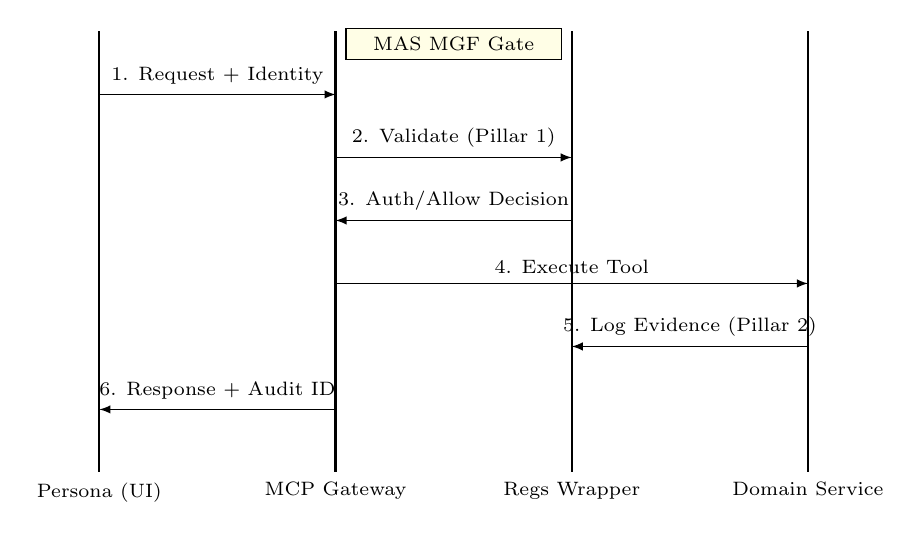
\begin{tikzpicture}[x=1cm, y=-0.8cm, font=\scriptsize]
    % Lifelines
    \draw[thick] (0,0) -- (0,7) node[below] {Persona (UI)};
    \draw[thick] (3,0) -- (3,7) node[below] {MCP Gateway};
    \draw[thick] (6,0) -- (6,7) node[below] {Regs Wrapper};
    \draw[thick] (9,0) -- (9,7) node[below] {Domain Service};

    % Interaction
    \draw[->, >=latex] (0,1) -- node[above] {1. Request + Identity} (3,1);
    \draw[->, >=latex] (3,2) -- node[above] {2. Validate (Pillar 1)} (6,2);
    \draw[<-, >=latex] (3,3) -- node[above] {3. Auth/Allow Decision} (6,3);
    \draw[->, >=latex] (3,4) -- node[above] {4. Execute Tool} (9,4);
    \draw[->, >=latex] (9,5) -- node[above] {5. Log Evidence (Pillar 2)} (6,5);
    \draw[<-, >=latex] (0,6) -- node[above] {6. Response + Audit ID} (3,6);

    \node[draw, fill=yellow!10, text width=2.5cm, align=center] at (4.5,0.2) {MAS MGF Gate};
\end{tikzpicture}
\caption{Standard platform handshake for governed tool execution. Audit schemas are detailed in \cref{reg:ch:identity}.}
\end{figure}

\subsection{Arabic AP Golden Path}
Temporal flow for invoice processing with Arabic context.

\begin{figure}[htbp]
\centering
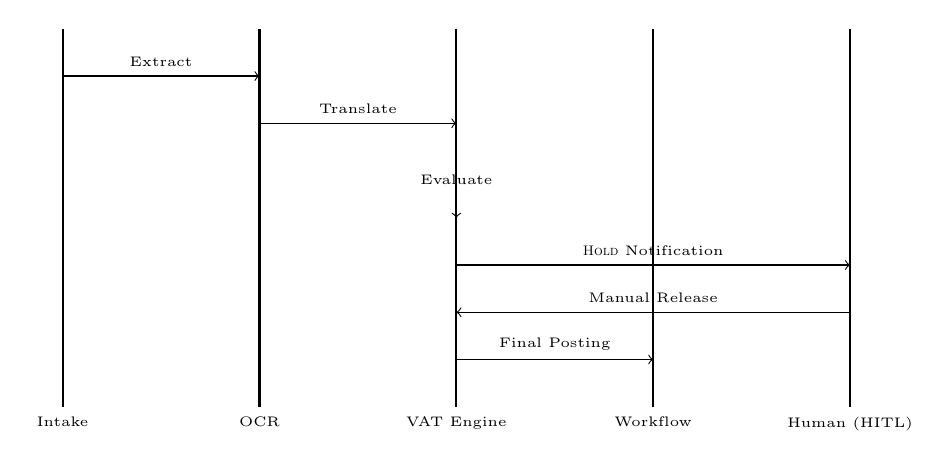
\begin{tikzpicture}[x=1cm, y=-0.6cm, font=\tiny]
    \draw[thick] (0,0) -- (0,8) node[below] {Intake};
    \draw[thick] (2.5,0) -- (2.5,8) node[below] {OCR};
    \draw[thick] (5,0) -- (5,8) node[below] {VAT Engine};
    \draw[thick] (7.5,0) -- (7.5,8) node[below] {Workflow};
    \draw[thick] (10,0) -- (10,8) node[below] {Human (HITL)};

    \draw[->] (0,1) -- node[above] {Extract} (2.5,1);
    \draw[->] (2.5,2) -- node[above] {Translate} (5,2);
    \draw[->] (5,3) -- node[above] {Evaluate} (5,4); % Internal loop
    \draw[->] (5,5) -- node[above] {\textsc{Hold} Notification} (10,5);
    \draw[<-] (5,6) -- node[above] {Manual Release} (10,6);
    \draw[->] (5,7) -- node[above] {Final Posting} (7.5,7);
\end{tikzpicture}
\caption{Arabic AP sequence: Scanned PDF to Release. VAT rules are specified in \cref{ar:ch:vat}.}
\end{figure}

\section{Compute and Resource Alignment}
\label{sec:hardware-profiles}

AI algorithms are calibrated for the reference infrastructure established in the domain chapters:

\begin{table}[htbp]
\centering
\footnotesize
\caption{Infrastructure Reference Profiles.}
\label{tab:hardware-profiles}
\begin{tabularx}{\textwidth}{@{}l X X@{}}
\toprule
\textbf{Workload} & \textbf{Reference Hardware} & \textbf{Performance Target} \\
\midrule
LLM Inference & NVIDIA L40S (48GB) & AWQ 4-bit / p95 < 2s \\
Embeddings & NVIDIA A100 (40/80GB) & FP16 / p99 < 500ms \\
Simula Training & NVIDIA A100 SXM4 cluster & BF16 throughput parity \\
\bottomrule
\end{tabularx}
\end{table}

\section{Human-in-the-Loop (HITL) Critical Gates}
\label{sec:hitl-gates}

The following "Four-Eyes" gates are mandatory. AI agents must implement the "Awaiting Sign-off" state for these actions:
\begin{itemize}
    \item \textbf{VAT Release:} No invoice marked as \textsc{hold} can be released without human review (see \cref{ar:ch:ap}).
    \item \textbf{Anomaly Override:} Statistical outliers ($3\sigma$) cannot be dismissed by AI; only "Confirmed" or "Triaged" by human (see \cref{tb:ch:controls}).
    \item \textbf{Journal Posting:} Agents may \emph{draft} journal entries, but only the Financial Controller persona can \emph{commit} to S/4HANA (see \cref{tb:ch:controls-engine}).
\end{itemize}

\section{Registry Integrity \& Live Status}
\label{sec:registry-integrity}

Before initiating any schema-dependent task, implementation agents must verify the live status of the Unified Schema Registry (see \cref{sim:chap:schema}).
\begin{adrbox}{Registry First}
If \texttt{docs/schema/registry.json} is out of sync with the codebase, the agent must halt and emit a \textsc{schema-mismatch} event.
\end{adrbox}

\section{Master Implementation Manifest (Union)}
Implementation runs in three waves across the entire platform.

\subsection*{Wave 1 --- Foundations}
\begin{itemize}
    \item \textbf{Simula:} Implement HANA schema extraction pipeline (MCP discovery). See \cref{sim:chap:extraction}.
    \item \textbf{Regulations:} Implement MAS MGF Pillar 1 logic (Tool allow-list). See \cref{reg:ch:mgf}.
    \item \textbf{Arabic:} Implement Invoice Intake \& OCR Gateway. See \cref{ar:ch:ai}.
    \item \textbf{Trial Balance:} Implement identity-attribution wiring. See \cref{reg:ch:identity}.
\end{itemize}

\subsection*{Wave 2 --- Core Domain Build-out}
\begin{itemize}
    \item \textbf{Trial Balance:} Implement Controls \& Commentary Engine (3$\sigma$ anomaly logic). See \cref{tb:ch:ai,tb:ch:controls-engine}.
    \item \textbf{Arabic:} Implement multi-country VAT Engine (Saudi, UAE, Bahrain, Oman). See \cref{ar:ch:vat,ar:ch:vat-impl}.
    \item \textbf{Simula:} Implement Taxonomy Generation \& Agentic Data Synthesis. See \cref{sim:chap:taxonomy,sim:chap:generator}.
    \item \textbf{Trial Balance:} Realise 28-state BPMN workflow (\texttt{tb-review-glo}). See \cref{tb:ch:workflow}.
\end{itemize}

\subsection*{Wave 3 --- Hardening}
\begin{itemize}
    \item \textbf{Regulations:} Implement Per-Request Identity Attribution. See \cref{reg:ch:identity}.
    \item \textbf{Trial Balance:} Deliver Human Review Dashboard. See \cref{tb:ch:review-dashboard}.
    \item \textbf{Simula:} Deliver test fixtures and testing at 85\% coverage. See \cref{sim:ch:test-fixtures,sim:ch:testing}.
    \item \textbf{Regulations:} Wire Emergent-Capability monitoring. See \cref{reg:ch:monitoring}.
\end{itemize}

\section{Governance Obligations (MAS MGF)}
The regulations domain wraps all service calls at runtime. Agents must implement the following hooks in every domain:
\begin{itemize}
    \item \textbf{Pillar 1:} Tool allow-list enforcement (deny-by-default).
    \item \textbf{Pillar 2:} Traceability via the identity attribution envelope.
    \item \textbf{Pillar 3:} Metric emission to the monitoring sink.
\end{itemize}
Detailed pillar requirements are defined in \cref{reg:ch:mgf}.


\section{FMEA: Failure Mode and Effects Analysis for AI}
\label{sec:fmea-ai}

The following analysis identifies critical AI failure modes within the Regulations governance runtime and their deterministic mitigations.

\begin{table}[htbp]
\centering
\footnotesize
\caption{FMEA for Regulations AI Governance Pipeline.}
\label{tab:reg-fmea}
\begin{tabularx}{\textwidth}{@{}l X X X@{}}
\toprule
\textbf{Failure Mode} & \textbf{Symptom} & \textbf{Impact} & \textbf{Technical Mitigation} \\
\midrule
Entitlement Drift & Persona allowed to call a non-allow-listed MCP tool. & Critical (Security) & Deny-by-default hard gate in MCP Gateway middleware. \\
Audit Omission & High-risk action emitted without Identity Envelope. & High (Compliance) & Mandatory envelope-check hook in PAL evidence-writer. \\
Monitoring Blindspot & Emergent capability detected but metrics not emitted. & Medium (Risk) & Periodic 'Heartbeat' probe to Monitoring Sink. \\
\bottomrule
\end{tabularx}
\end{table}

\section{This domain in context}
\label{sec:agent-domain-context}
Regulations is unique among the four domains: it is both a persona
surface (Compliance Officer) and the horizontal runtime wrapper that
governs Arabic, TB, and Simula at every MCP call. As a persona
surface, its working view is the governance dashboard surfaced
through the shared workspace shell and gated by regulations
entitlements. As a runtime wrapper, it has no separate service of
its own: the governance hooks are attached to the gateway and to
ai-core-pal, and they are exercised on every call the platform
handles. Its entry points are (a)~any inbound MCP call into any
domain, which must pass through the governance gate, and (b)~the
Compliance Officer's review queue. Its exit points are
(a)~governance decisions (allow, deny, degrade) returned to the
gateway, (b)~evidence records written to the shared governance
store, and (c)~conformance reports for auditors.

\section{Schema contribution}
\label{sec:agent-schema-contrib}
Regulations owns the schemas catalogued in chapter~\ref{ch:schema}
and listed in~\ref{tab:schemas}. The canonical set is the
requirement record (the linkage schema between source rule, artefact,
and evidence), the conformance-tool record, the enum vocabularies
in~\ref{tab:enums}, the capability-monitoring metrics record
(chapter~\ref{ch:monitoring}), and the identity and audit-event
schemas in chapter~\ref{ch:identity}. These schemas live under
\texttt{docs/latex/specs/regulations/} as normative text and under
\texttt{structured/schema/} as the JSON Schema artefacts consumed at
runtime. Registration in the unified registry is additive: each
schema is listed in
\texttt{src/intelligence/ai-core-pal/data\_products/registry.yaml}
with its URI, owning domain (\texttt{regulations}), security class
(\texttt{confidential}), and LLM routing (\texttt{vllm-only}),
following the ODPS~4.1 pattern. Simula consumes these schemas
directly as inputs to its extraction pipeline; it does not transform
them. Regulations' \texttt{requirement.schema.json} is a distinct
URI from TB's \texttt{requirement.schema.json}; the two files are
not merged.

\section{Persona and MCP allow-list}
\label{sec:agent-persona}
\begin{itemize}
  \item \textbf{Persona id:} \texttt{compliance-officer}.
  \item \textbf{Roles:} requirement registration, governance-policy
    authoring, conformance-run triage, emergent-capability review,
    audit-trail inspection.
  \item \textbf{Entitlements:} read/write on the requirement record,
    conformance-tool record, capability-monitoring record, and the
    identity-and-audit schemas; read on every other domain's
    evidence output (needed to assemble conformance reports);
    override-write on governance-decision records (rare, audit-logged).
  \item \textbf{UI route:} \texttt{/governance/\{tenant\}/dashboard}
    on the shared workspace shell; surfaced only to callers whose
    entitlement set includes \texttt{compliance-officer}.
  \item \textbf{MCP tool allow-list:}
    \texttt{gov.requirement.register}, \texttt{gov.policy.publish},
    \texttt{gov.conformance.run}, \texttt{gov.conformance.report},
    \texttt{gov.monitor.query}, \texttt{gov.audit.query},
    \texttt{gov.identity.attest}. All other MCP tools are denied by
    default per MAS MGF pillar~1.
\end{itemize}

\section{Agent Rule-Pack Binding}
\label{sec:agent-rule-binding}
Before initiating any task in this domain, the agent MUST load the following rule packs in order:
\begin{enumerate}
  \item \filepath{.clinerules} (Global Standards)
  \item \filepath{src/intelligence/.clinerules} (Regulations Envelope)
\end{enumerate}

\section{Implementation tasks for this domain}
\label{sec:agent-tasks}
The tasks below are intent-based: each task states the outcome a
future agent must achieve and the location in the existing codebase
where the work belongs. None of them contains code; each task binds
to the regulations chapters that define the required behaviour.

\subsection*{Task R1 --- MGF four-pillar runtime checks}
\textbf{Intent.} Realise the four MAS MGF pillars defined in
chapter~\ref{ch:mgf} as runtime checks that run on every inbound MCP
call in every non-regulations domain.

\begin{adrbox}{Why Pillars over Flat Rules?}
We adopted the MAS MGF Pillar structure to ensure that governance is not just a 'checklist' but a runtime operational model that scales as new domains (e.g., ESG, Supply Chain) are onboarded.
\end{adrbox}

\textbf{In-scope.} Pillar~1 (assess and bound) via allow-list
enforcement at the gateway; pillars~2--4 via the evidence and
disclosure hooks on ai-core-pal; pillar binding per
\S\ref{sec:mgf-p1} and~\ref{tab:p1}.
\textbf{Out-of-scope.} Re-implementing the MGF rule source; the
source document is frozen and referenced by its sha in~\ref{tab:src-hashes}.
\textbf{Paths to extend.} Governance hooks in the gateway; evidence
writer in ai-core-pal.
\textbf{Definition of done.} Every allow/deny decision references a
pillar; denials are surfaced to the caller with a stable error code;
evidence records for each pillar are written for every call.

\textbf{Autonomous Verification (Agent Logic):}
\begin{lstlisting}[language=jsonx]
// Verify Task R1
{
  "test_fixture": "tests/fixtures/regulations/unauthorized_call.json",
  "expected_outcome": "http_status == 403",
  "validation_command": "make test-gov-runtime --pillar=1"
}
\end{lstlisting}

\textbf{Verification.} Running any non-regulations domain's golden
sample produces a governance evidence record per pillar per call;
\texttt{make spec-regulations} remains green.

\subsection*{Task R2 --- AI Agent Index mapping}
\textbf{Intent.} Operationalise the 2025 AI Agent Index
transparency requirements listed in chapter~\ref{ch:agent-index},
especially~\ref{tab:agentidx-reqs}.
\textbf{In-scope.} Requirement registration per row; verification
runners that check that each agent surface exposes the required
transparency metadata (model, training set summary, known failure
modes).
\textbf{Out-of-scope.} Public disclosure portals.
\textbf{Paths to extend.} Requirement record loader; governance
dashboard transparency tab.
\textbf{Definition of done.} Every row in~\ref{tab:agentidx-reqs}
maps to a runnable verification; failures show up on the dashboard.
\textbf{Verification.} Conformance runner report 100\% of Agent
Index requirements either passing or explicitly waived with
attached evidence.

\subsection*{Task R3 --- Empirical evaluation hookup}
\textbf{Intent.} Encode the requirements extracted from Ju \& Aral
(2026) in chapter~\ref{ch:empirical} and~\ref{tab:jural-reqs} as
runnable empirical checks against the platform.
\textbf{In-scope.} Test harness that executes the Ju \& Aral
requirements on Arabic, TB, and Simula outputs; periodic run
cadence.
\textbf{Out-of-scope.} Adding new empirical studies.
\textbf{Paths to extend.} Regulations test harness colocated with
chapter~\ref{ch:testing} fixtures; scheduler hook.
\textbf{Definition of done.} Every requirement
in~\ref{tab:jural-reqs} has a callable check; the harness reports
pass/fail per requirement on the most recent platform build.
\textbf{Verification.} Harness run produces a per-requirement
report; failures block the CI gate.

\subsection*{Task R4 --- Conformance tooling integration}
\textbf{Intent.} Integrate AI Verify 2.0 and Moonshot CI/CD 1.1.0
per chapter~\ref{ch:tooling} and the coverage map
in~\ref{fig:tool-coverage}.
\textbf{In-scope.} AI Verify plug-ins listed in~\ref{tab:av-plugins}
and Moonshot benchmarks listed in~\ref{tab:ms-benchmarks};
conformance-run CLI exposed to the Compliance Officer persona.
\textbf{Out-of-scope.} Upstream changes to AI Verify or Moonshot.
\textbf{Paths to extend.} Conformance harness invoked from the
gateway; dashboard run-history view.
\textbf{Definition of done.} Running the conformance suite against
the platform produces a unified report covering every plug-in and
every benchmark in the two tables.
\textbf{Verification.} \texttt{gov.conformance.run} returns a report
that validates against the conformance-tool schema.

\subsection*{Task R5 --- Capability monitoring}
\textbf{Intent.} Deliver the capability monitoring specification in
chapter~\ref{ch:monitoring}, with the architecture
in~\ref{fig:monitor-arch} and the metrics in~\ref{tab:monitor-metrics}.
\textbf{In-scope.} Metrics collection at each of the collection
points; storage in the monitoring sink; threshold-based alerts.
\textbf{Out-of-scope.} Long-term analytics warehouse.
\textbf{Paths to extend.} Monitoring hooks on ai-core-pal; alert
router.
\textbf{Definition of done.} Every metric in~\ref{tab:monitor-metrics}
is emitted in production; alerts fire on the thresholds the chapter
defines.
\textbf{Verification.} Synthetic load test shows every required
metric at the sink; alerting simulator triggers every configured
alert.

\subsection*{Task R6 --- Identity attribution}
\textbf{Intent.} Realise per-request identity attribution per
chapter~\ref{ch:identity}, including the agent identity, request
identity, and audit-event schemas.
\textbf{In-scope.} Identity envelope construction at the gateway;
propagation through every domain service call; audit writer that
emits every required event.
\textbf{Out-of-scope.} Replacing the existing authentication
backend.
\textbf{Paths to extend.} Gateway identity middleware; audit writer
in ai-core-pal.
\textbf{Definition of done.} No MCP call leaves the gateway without
a complete identity envelope; every required audit event is written
with the schema's required fields.
\textbf{Verification.} Audit query over a test run surfaces every
event class; absent or partial envelopes fail the CI gate.

\subsection*{Task R7 --- Testing}
\textbf{Intent.} Deliver the regulations testing specification in
chapter~\ref{ch:testing} at the coverage thresholds
in~\ref{tab:reg-coverage}.
\textbf{In-scope.} Regulation fixtures, conformance-tool fixtures,
unit tests for requirement parsing, integration tests over the
governance gate.
\textbf{Out-of-scope.} Load benchmarking beyond what
chapter~\ref{ch:testing} defines.
\textbf{Paths to extend.} Test directory colocated with the
regulations service code.
\textbf{Definition of done.} Coverage meets~\ref{tab:reg-coverage};
CI gates block regressions.
\textbf{Verification.} \texttt{make spec-regulations} remains green;
the regulations test entry points all run.


\section{Governance obligations applied to this domain}
\label{sec:agent-governance}
Regulations is both the persona surface and the wrapper. The four
obligations therefore apply to regulations in two ways: as the
author of the obligations (canonical source in this spec's chapters)
and as a subject of the obligations (like every other domain, its
own MCP calls pass through the governance gate).

\begin{itemize}
  \item \textbf{MAS MGF four pillars} (chapter~\ref{ch:mgf}). The
    regulations service authors the pillar definitions; it also
    executes them against its own MCP tools. Pillar~1 enforcement
    applies the allow-list in \S\ref{sec:agent-persona},
    deny-by-default.
  \item \textbf{Identity attribution} (chapter~\ref{ch:identity}).
    Regulations owns the identity and audit-event schemas; its own
    MCP calls carry the identity envelope like any other domain.
  \item \textbf{Emergent-capability monitoring}
    (chapter~\ref{ch:monitoring}). Regulations authors the metrics
    model; governance decisions, conformance runs, and audit queries
    are themselves instrumented.
  \item \textbf{Conformance tooling} (chapter~\ref{ch:tooling}).
    Regulations integrates AI Verify 2.0 and Moonshot CI/CD 1.1.0
    as runnable suites; the regulations service's own behaviour is
    included in every conformance run.
\end{itemize}

\section{Cross-spec integration --- full detail}
\label{sec:agent-integration}

\subsection{With Arabic AP}
Regulations wraps Arabic at runtime. Every Arabic MCP call is
brokered through the regulations governance gate, which applies
pillars~1--4 of MAS MGF, attaches the identity envelope, and routes
emergent-capability metrics to the monitoring store. Arabic exports
the invoice record, VAT compliance checklist, and payment
instruction schemas under \texttt{structured/schema/} and registers
its MCP tools with the gateway; the governance gate consumes those
registrations but adds no Arabic-specific code paths. Conformance
tests defined here execute against the Arabic service as part of
the platform CI gate.

\subsection{With Trial Balance}
Regulations wraps TB at runtime. Every TB MCP call is brokered
through the regulations governance gate, which applies pillars~1--4
of MAS MGF, attaches the identity envelope, and routes
emergent-capability metrics to the monitoring store. TB exports the
control record, decision-point record, workflow record, and its own
\texttt{requirement.schema.json} under \texttt{structured/schema/}.
Regulations' \texttt{requirement.schema.json} is a distinct URI
from TB's; no schema merge takes place.

\subsection{With Regulations}
Regulations exports the requirement record, conformance-tool record,
enum vocabularies, capability-monitoring metrics record, and the
identity and audit-event schemas under \texttt{structured/schema/};
registers the MCP tools enumerated in \S\ref{sec:agent-persona};
and applies the four governance hooks in
\S\ref{sec:agent-governance} to every call it serves --- including
its own. External consumers (Arabic, TB, Simula) see regulations
only through these contracts and through the wrapper; there are no
private back-channels.

\subsection{With Simula}
Regulations wraps Simula at runtime in the same way it wraps Arabic
and TB. Simula also consumes regulations' schemas (requirement,
conformance-tool, monitoring metrics, identity and audit) as
training input. The contract is schema-in,
\texttt{TrainingExample}-out: Simula reads the regulations schema
set; it produces \texttt{TrainingExample} records. Simula does not
call regulations MCP tools at runtime and does not share state with
the governance dashboard. No cross-domain operational envelope is
introduced.

\section{Wave assignment and sequencing}
\label{sec:agent-waves}
Implementation runs in three waves.

\begin{itemize}
  \item \textbf{Wave 1 --- foundations.} Identity schema
    (chapter~\ref{ch:identity}) frozen; gateway identity envelope;
    persona-gated surface for the Compliance Officer; unified schema
    registry entries for regulations schemas.
  \item \textbf{Wave 2 --- governance runtime.} Tasks R1, R4, R5, R6
    above. Prerequisites: Wave~1 complete; Simula Wave~1 extraction
    pipeline available for monitoring metrics ingestion.
  \item \textbf{Wave 3 --- evaluation and hardening.} Tasks R2, R3,
    R7. Prerequisites: Wave~2 complete; monitoring sink live; all
    non-regulations domains exposing their conformance entry
    points.
\end{itemize}

Regulations is the critical-path domain for Wave~1 (identity) and
Wave~2 (governance runtime). Other domains block on regulations'
Wave~1 completion.

\section{Acceptance criteria (platform-wide)}
\label{sec:agent-acceptance}
When all four chapter~12 instruction sets are implemented, the
platform satisfies the following invariants:

\begin{enumerate}
  \item \textbf{One instance.} A single codebase runs a single
    logical instance; no domain ships as a separate product.
  \item \textbf{Persona-gated surfaces.} The four personas each
    reach a tailored UI on the shared shell; no route, MCP tool, or
    data product is visible outside its persona's entitlement set.
  \item \textbf{Unified registry.} Every schema in use is listed in
    the ODPS~4.1 registry under its owning domain; validators
    resolve \texttt{\$ref}s through the unified registry only.
  \item \textbf{No schema merges.} The two
    \texttt{requirement.schema.json} files in TB and regulations
    remain distinct; no cross-domain composite schemas are produced.
  \item \textbf{No cross-domain operational envelope.} Runtime
    orchestration stays within each domain's service; only Simula
    consumes other domains' outputs, and only as training input.
  \item \textbf{Governance wraps all three non-regulations domains.}
    Arabic, TB, and Simula service calls pass through the
    regulations runtime wrapper without exception.
\end{enumerate}

\section{References}
\label{sec:agent-references}
Within-spec references:
chapter~\ref{ch:overview} (overview),
chapter~\ref{ch:schema} (data schema),
chapter~\ref{ch:mgf} (MAS MGF framework),
chapter~\ref{ch:agent-index} (AI Agent Index),
chapter~\ref{ch:empirical} (Ju \& Aral empirical evidence),
chapter~\ref{ch:tooling} (conformance tooling),
chapter~\ref{ch:refs} (references and traceability),
chapter~\ref{ch:monitoring} (capability monitoring),
chapter~\ref{ch:testing} (testing specification),
chapter~\ref{ch:identity} (identity attribution),
chapter~\ref{ch:reg-roadmap} (project roadmap).

Peer chapter~12 instruction sets for the other three domains (each
is self-contained; consult directly when operating in that domain):
\begin{itemize}
  \item Arabic AP:
    \texttt{docs/latex/specs/arabic/chapters/12-implementation-instructions.tex}.
  \item Trial Balance:
    \texttt{docs/latex/specs/tb/chapters/12-implementation-instructions.tex}.
  \item Simula:
    \texttt{docs/latex/specs/simula/chapters/12-implementation-instructions.tex}.
\end{itemize}

Shared platform artefacts:
\begin{itemize}
  \item ODPS~4.1 registry:
    \texttt{src/intelligence/ai-core-pal/data\_products/registry.yaml}.
  \item Schema pipeline and resolver:
    \texttt{src/intelligence/schema\_pipeline/}.
  \item Training pipeline (Simula):
    \texttt{src/training/pipeline/}.
  \item Shared workspace shell:
    \texttt{generativeUI/training-webcomponents-ngx}.
\end{itemize}
